
\documentclass[11pt,a4paper,sans]{moderncv}        % possible options include font size ('10pt', '11pt' and '12pt'), paper size ('a4paper', 'letterpaper', 'a5paper', 'legalpaper', 'executivepaper' and 'landscape') and font family ('sans' and 'roman')

% moderncv themes
\moderncvstyle{classic}                            % style options are 'casual' (default), 'classic', 'oldstyle' and 'banking'
\moderncvcolor{blue}                               % color options 'blue' (default), 'orange', 'green', 'red', 'purple', 'grey' and 'black'
%\renewcommand{\familydefault}{\sfdefault}         % to set the default font; use '\sfdefault' for the default sans serif font, '\rmdefault' for the default roman one, or any tex font name
%\nopagenumbers{}                                  % uncomment to suppress automatic page numbering for CVs longer than one page


\makeatletter
\renewcommand*{\bibliographyitemlabel}{\@biblabel{\arabic{enumiv}}}
\makeatother

% adjust the page margins
\usepackage[scale=0.765]{geometry}
\setlength{\hintscolumnwidth}{2.04cm}                % if you want to change the width of the column with the dates
%\setlength{\makecvtitlenamewidth}{10cm}           % for the 'classic' style, if you want to force the width allocated to your name and avoid line breaks. be careful though, the length is normally calculated to avoid any overlap with your personal info; use this at your own typographical risks...

%%%%%%%%%%%%%%% Nasty hack to avoid whitespace before the bib
%\makeatletter
%\renewenvironment{thebibliography}[1]{%
%     \section*{\refname}%
%      \@mkboth{\MakeUppercase\refname}{\MakeUppercase\refname}%
%      \list{\@biblabel{\@arabic\c@enumiv}}%
%           {\settowidth\labelwidth{\@biblabel{#1}}%
%            \leftmargin\hintscolumnwidth
%            \advance\leftmargin\labelsep
%            \@openbib@code
%            \usecounter{enumiv}%
%            \let\p@enumiv\@empty
%            \renewcommand\theenumiv{\@arabic\c@enumiv}}%
%      \sloppy
%      \clubpenalty4000
%      \@clubpenalty \clubpenalty
%      \widowpenalty4000%
%      \sfcode`\.\@m}
%     {\def\@noitemerr
%       {\@latex@warning{Empty `thebibliography' environment}}%
%      \endlist}
%\makeatother
%
\usepackage[normalem]{ulem}
\usepackage{color}
\usepackage{bm}
\usepackage{amstext}
\usepackage{amssymb}
\newcommand{\coloredLink}[2]{\textcolor{blue}{\href{#1}{#2}}}
\usepackage{tikzpagenodes}


\newcommand\ttbb{\ensuremath{t\bar{t}b\bar{b}}}
\newcommand\ttbar{\ensuremath{t\bar{t}}}
\newcommand\tttt{\ensuremath{t\bar{t}t\bar{t}}}
\newcommand\ttH{\ensuremath{t\bar{t}H}}
\newcommand\ttZ{\ensuremath{t\bar{t}Z}}
\newcommand\ttW{\ensuremath{t\bar{t}W}}
\newcommand\bbbar{\ensuremath{b\bar{b}}}
\newcommand{\met}{\ensuremath{E_{{T}}^{{miss}}}}
\newcommand{\pt}{\ensuremath{p_{T}}}

\newif\ifAddReferences  %% References
\newif\ifAddStatement  %% Statement of research interest
\newif\ifAddTeaching  %% Teaching statement
\newif\ifAddInternalTalks  %% References
\newif\ifAddTalks  %% References
\AddReferencesfalse
\AddStatementfalse
\AddTeachingfalse
\AddInternalTalksfalse
\AddTalkstrue

\AtBeginDocument{\hypersetup{colorlinks,citecolor=blue,linkcolor=blue,urlcolor=blue}}
\AtBeginDocument{\renewcommand\refname{~}}

\name{Javier}{Montejo Berlingen} %many FIXME around the CV, find them
%%%%%%%%%%%%%%%%%%%%%%
% SINCE YOU ARE READING THIS, LET ME REMIND YOU ABOUT THE IDEA OF HAVING A VERTICAL LINE IN THE MIDDLE
% AND THE RESULTS AND POSITIONS ON BOTH SIDES TO GIVE CONTEXT OF THE TIMELINE
%                                                                  CHECK 'CV nuevo layout.key' <----------
%%%%%%%%%%%%%%%%%%%%%%
\title{CERN Staff Physicist}                               % optional, remove / comment the line if not wanted
%\address{CERN 40/5-C11}{1217 Meyrin}{Switzerland}
%\phone[fixed]{+41~786314562}
%\email{jmontejo@cern.ch}                               % optional, remove / comment the line if not wanted


\usepackage{multibib}
\newcites{article,confnote,proceedings}{{Articles},{Conference Notes},{Proceedings}}

%----------------------------------------------------------------------------------
%            content
%----------------------------------------------------------------------------------
\begin{document}
%-----       resume       ---------------------------------------------------------
\makecvtitle
\vspace*{-15mm}

\begin{tikzpicture}[remember picture,overlay,shift={(current page.north east)}]
\node[anchor=north east,xshift=-2cm,yshift=-2.3cm]{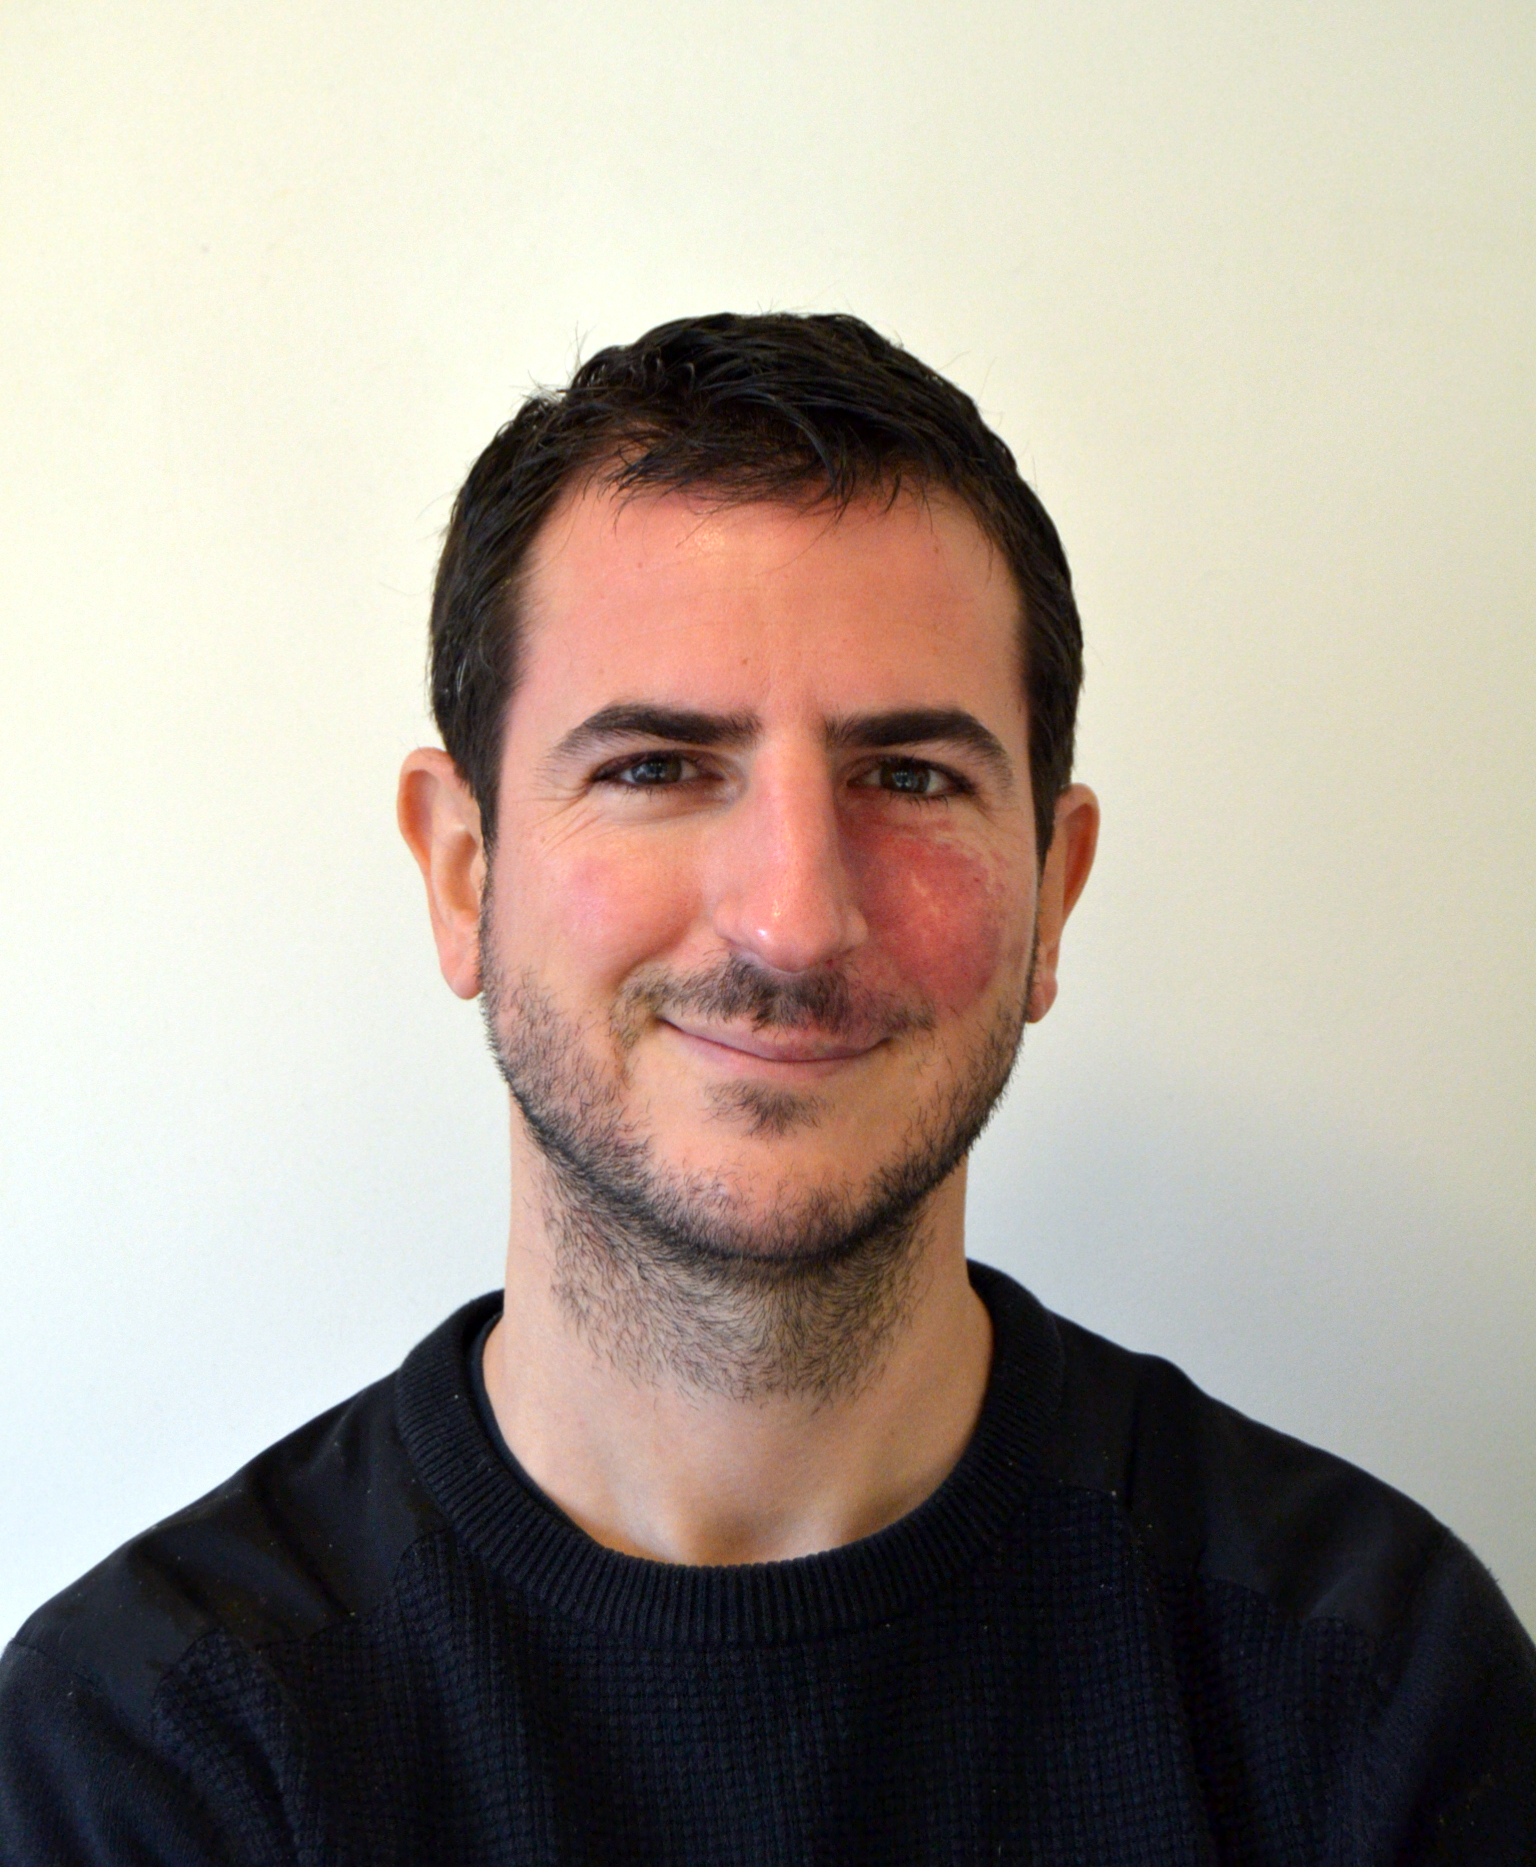
\includegraphics[width=5cm]{Javi_foto_curriculum_gimp_crop}};
\end{tikzpicture}

\section{Personal Information}
\cvline{Date of birth}{March 26, 1986}
%\cvline{Place of birth}{Salamanca, Spain}
%\cvline{Sex}{Male}
\cvline{Nationality}{Spanish, German}
\cvline{Email}{jmontejo@cern.ch}
\cvline{Phone}{+41 786314562}
\cvline{ORCID}{0000-0001-9213-904X}

\vspace*{5mm}


\section{Education and Research Positions}
\cventry{2017 - today}{CERN Staff Physicist}{}{}{
\newline{}LHC LLP working group convener.
\newline{}SUSY R-parity violating and long-lived subgroup convener.
\newline{}Trigger Level-1 calorimeter algorithm and performance coordinator.
\newline{}Trigger menu and performance coordinator. 
\newline{}Member of Physics Coordination group.
\newline{}Member and Scientific Secretary of the Trigger Coordination Group.
\newline{}Supervisor of two CERN fellows.}{}
%FIXME Reviewer for EPJC and polish grants
\cventry{2015 - 2017}{CERN Fellow}{}{}{\newline{}SUSY third-generation subgroup convener.}{}
\cventry{2012 - 2015}{Ph.D.,}{Universitat Aut\'onoma de Barcelona,}{Spain.}{\newline{}
UAB physics thesis award.\newline{}ATLAS thesis award.\newline{}Springer thesis award.}{}
\cventry{2011 - 2012}{M.Sc. in High-Energy Physics,}{Universitat Aut\'onoma de Barcelona,}{Spain.}{}{}
\cventry{2005 - 2011}{B.Sc. in Computer Science,}{Universidad de Salamanca,}{Spain.}{\newline{}
Extraordinary Graduation Award.}{}
\cventry{2005 - 2010}{B.Sc. in Physics,}{Universidad de Salamanca,}{Spain.}{\newline{}Extraordinary Graduation Award.\newline{}National Award for Excellence in Academic Performance.}{}{}

\section{Outreach and mentoring}
%FIXME Romanian summer school
\cvitem{}{Discussion leader at the 2021 CERN-Fermilab Hadron Collider Physics Summer School.}
\cvitem{}{Beamline for schools (B4LS) 2020, assistant and analysis support.}
\cvitem{}{International masterclass 2016--2018, moderator and virtual visits.}
%\cvitem{}{World of work 2018, host and supervisor.}
\cvitem{}{Supervisor of three summer students, 2016--2019}
\cvitem{}{ATLAS guide since 2015.}


\clearpage
\section{Research Experience}

\cvitem{}{
I have developed my research career in the field of experimental high energy physics, working in the ATLAS experiment at the LHC accelerator at CERN. I was awarded with a FPU grant and obtained my PhD from the Universidad Autónoma de Barcelona in 2015 with Cum Laude honors. 
}
%%%%%%%%%%%%%%%% ttH(bb)
\cvitem{Run~1:}{
Throughout my career, I have worked on physics analyses targeting different aspects of the hierarchy problem. During my PhD I was the lead analyser for the first searches for ttH, which led to the confirmation of the SM-like nature of the top Yukawa coupling~\cite{HIGG-2013-27}. I then transitioned to searches for beyond-the-standard-model top partners, that could cancel the top-loop corrections to the Higgs mass. I developed the first search for vector-like tops decaying to Higgs bosons, covering for the first time the full spectrum of possible decays~\cite{EXOT-2013-18}. I also performed a search for supersymmetric top partners, targeting the production of the heavier stop and the subsequent decay to the lightest stop and Higgs boson ($\tilde{t}_2 \rightarrow \tilde{t}_1 H$)~\cite{SUSY-2014-07}.
}
\cvitem{}{
During this period I also worked on the characterisation and calibration of the timing performance of the Tile calorimeter using collision data. I identified multiple detector and geometrical effects that were previously not accounted for, and introduced a set of selection cuts and corrections that improved the resolution of the time measurement by up to 20\%~\cite{TCAL-2017-01}. 
}

\cvitem{{RPC SUSY}}{
After my PhD I obtained a CERN research fellowship. During this time, I led a series of searches for scalar top partners, redesigning the search for a much better performance. The strong sensitivity and flexibility of the analysis led to a series of publications with integrated luminosities of 3.2~fb$^{-1}$\cite{SUSY-2015-02}, 14 fb$^{-1}$\cite{ATLAS-CONF-2016-050} and 36 fb$^{-1}$\cite{SUSY-2016-16}, with increasingly comprehensive coverage of stop production within natural SUSY scenarios. As recognition of my work I was appointed convener of the third-generation supersymmetry group.  
}

\cvitem{Trigger}{
Alongside physics analysis, I have been heavily involved in the trigger group where I have contributed to the operation, development and design of the trigger menu, which defines the data that is recorded by ATLAS. I was appointed as trigger menu and signature coordinator, and as such I was part of the Trigger Coordination board, as well as the Physics Coordination board, the most important body in ATLAS concerning all topics related to the physics research programme. In this position I was in charge of the physics, detector, and signature trigger subgroups, comprising more than a hundred members. I also had the pleasure of defining the Run 3 ATLAS trigger menu, shaping the physics programme of the experiment for next years. 
}
\cvitem{{RPV SUSY and LLPs}}{
I am currently CERN research staff, and during the last years I have transitioned to less common new physics searches, such as supersymmetric models with R-parity violation (RPV), or models with long-lived particles. I have developed a new search covering a gap in coverage pointed out by theorists, in the final state of one lepton and many jets~\cite{SUSY-2016-11}. In the second iteration, I introduced state-of-the-art machine learning techniques, that allowed to reach sensitivity to electroweak production. The analysis provides the first limits on higgsinos decaying via RPV since LEP~\cite{SUSY-2019-04}.}
\cvitem{}{
During this period I was appointed convener of the R-parity violating and long-lived supersymmetry group. I also initiated a taskforce to explore the interplay of RPC analyses, prompt RPV analyses, and long-lived searches~\cite{ATLAS-CONF-2018-003}. I am currently LHC LLP working group convener, where I coordinate the work of theorists and experimentalists studying long-lived particles across LHC experiments.
}

\cvitem{{BSM Higgs}}{
Possible additional decays of the Higgs boson are still compatible with current measurements, with branching ratios of up to $\mathcal{O}(10\%)$, as well as additional bosons from extended Higgs sectors. I have contributed to the design and optimisation of an analysis targeting the decay of the Higgs boson to two light pseudo-scalars, which in turn decay to pairs of b-quarks~\cite{HDBS-2018-47}. 
In addition, I am currently working on an analysis targeting models where the heavy Higgs sector can exhibit flavour-changing neutral currents. This kind of models feature a rich phenomenology, and can produce yet unexplored signatures such as three-top production.
}

\cvitem{Run~3}{
As part of my effort to improve the Run 3 triggers, I am currently coordinator of the Level-1 calorimeter algorithm and performance forum, where I am leading efforts to develop and optimise reconstruction and identification algorithms, in order to achieve the best possible performance out of the trigger phase-I upgrade.
}
\cvitem{}{
In summary, throughout my career in ATLAS I have performed measurements and searches within the Top, Higgs, Exotics and SUSY groups, targeting different aspects of the hierarchy problem. I have also contributed strongly in the Tile calorimeter and in the Trigger groups. During this time I have been entrusted with several management and coordination roles with an increasing level of responsibility and leadership, and proved my ability to lead large research groups in an international environment. 
}

\ifAddStatement
\clearpage
%\setlength{\hintscolumnwidth}{0cm}
%\setlength{\maincolumnwidth}{15.6cm}
\section{Statement of research interest}

%Warwick
%   Vcb through top decay
%   Higgs in gammagamma and bb states
%   fragmentation analysis in minimum bias events
%   searches for new Higgs bosons, including a long-lived A decaying to bb
%   high level trigger for high luminosity running
%   quality control and construction of strip modules for the Silicon Tracker upgrade.

%%%%%%%%% Intro and hierarchy probelm
\cvitem{}{
After the successful observation of the Higgs boson in Run 1, the increased energy of Run 2 has provided the LHC experiments with an unprecedented dataset to explore the energy frontier. No significant excess has been observed so far, and stringent limits have been set on simplified models.
The motivation for some form of new physics is still strong, but it is obvious that it is not manifested in the vanilla signatures that were the main focus of attention.
The Higgs boson mass has been measured at the electroweak scale, and the corresponding \emph{hierarchy problem} remains an unsolved question that I would like to address.
}

%%%%%%%%% Natural supersymmetry and RPV
\cvitem{}{
Natural supersymmetry remains a prime candidate to solve the hierarchy problem, and in particular R-parity violating (RPV) supersymmetry models can feature naturally light mass spectra with only weak exclusion limits. One of the key ingredients in natural supersymmetry is the presence of light higgsinos. Searches for higgsino production in final states with missing energy are well established at the LHC, and will continue progressing. However, higgsino searches without missing energy, as predicted by RPV, are largely uncovered. My goal is to develop a programme to cover the natural region of light higgsinos, including the most challenging decays. While the motivation to develop such programme originates as a search for higgsinos, the final states to be covered are sensitive to a large variety of BSM models.}
%Ewk production slepton-mediated > 1 TeV

%%%%%%%%% multi-lepton multi-bjet and LQD
\cvitem{}{
I have recently developed an analysis targeting higgsino production with RPV decay via a baryon-number-violating coupling $UDD$, exploiting the final state with at least one lepton and many $b$-jets ($\geq 1 \ell, \geq 3$ b-jets).
This search provides the first limits on hadronic higgsino decays since LEP. I would like to extend the analysis into the multi-leptons multi-$b$-jets final state ($\geq 3 \ell, \geq 3$ b-jets), in order to target also effectively decays via the lepton-number-violating coupling $LQD$, which is so far uncovered. 
Supersymmetric models with this coupling have received renewed interest recently given their potential to explain the $R_K$, $R_K^*$, and muon $g-2$ anomalies.
It is worth highlighting that searches in multi-lepton and multi-$b$-jets final states are not exclusive to RPV supersymmetry. Other models such as stealth supersymmetry or longer decay chains within the electroweak superpartners also predict similar final states, as well as non-supersymmetric models such as additional scalars or pseudoscalars in 2HDMs or vector-like quarks.
%A common aspect of these models is the possibility for higgsinos to decay via multiple vector bosons and higgs bosons or additional scalars, depleting the final state from \met. As part of the program, a search for b\=b resonances in this final state would tackle these kind of models. 
%Therefore, light higgsinos with such challenging decays have not been tested yet, and could also be accessed with the multi-lepton multi-$b$-jet final state.
Therefore, the multi-lepton multi-$b$-jet final state can be used to target a large variety of models that can populate this challenging final state.
}

%%%%%%%%% ttW+bb measurement
\cvitem{}{
This final state is certainly not new, and searches have already been performed, focusing however on high-mass signals. Typical requirements of $H_T$ or $m_{eff}$ around the TeV scale, or large \met\ make existing searches blind to low-mass signals.
For low-mass signals, the lack of striking distinguishing features requires an excellent control of the background modelling in order to fully capitalise on the possibilities of this channel.
The main background in this final state originates from \ttW\ with additional heavy flavour jets. %, and to a lesser extent \ttbar\ with additional fake or non-prompt leptons. 
Despite the availability of NLO predictions for the \ttW\ process, the modelling uncertainties on this background remain large, and several analyses observe data/MC disagreements above 50\%. Keeping in mind the long-term possibilities of this final state, I consider that a differential measurement of the \ttW\ process, in particular with additional heavy-flavour jets, is a required first step to establish the programme.
}

%%%%%%%%% long-lived 
\cvitem{}{
In order to achieve an exhaustive coverage of the higgsino landscape, a possibility that should not be neglected is that the higgsinos (or other BSM particles) could be long-lived. 
%The numerical values of the RPV couplings are often considered a free parameter of the theory. 
Searches for displaced decays, such as displaced vertices, have been conducted at the LHC, however focusing mostly on strong production. 
The selections and reconstruction techniques that target gluinos and R-hadrons above 2 TeV are extremely inefficient in the search for higgsinos at the electroweak scale. %they might be familiar with H 4b -like DVs
Searches for displaced decay products from low-mass scalars also exist, but rely on the associated production with a vector boson, which is not possible in the case of higgsinos or new pseudoscalars.
In addition, the background levels increase dramatically when attempting to adapt current searches towards vertices with lower masses and lower number of tracks, as required to have acceptance to lower mass scales.
Therefore, I would like to pursue a programme for electroweak-scale displaced decays, leading to displaced vertices. 
%And in particular, focusing on processes such as higgsino production, that do not benefit from the possibility of associated production with a vector boson. 
}

%%%%%%%% DV with soft muons
\cvitem{}{
From an experimental point of view, one of the main handles to identify the signals previously discussed was the presence of a high number of $b$-jets. This feature is seemingly lost when considering displaced decays. One possibility to recover it however, is to exploit B-hadron decays to muons. By requiring a displaced vertex with one or more muons attached, the backgrounds can be massively reduced, enabling a search for displaced vertices with lower masses and lower number of tracks. Other interesting signals that can be accessed lowering the track multiplicity requirements are for example decays of new pseudoscalars to two displaced taus, which are so far uncovered. The low production cross section and additional penalty from the muonic branching ratio of B-hadrons or taus requires a large recorded dataset, but the achieved purity can be excellent, making this a suitable target for the upcoming LHC runs. 
%
}

%%%%%%%% trigger
\cvitem{}{
One of the main challenges of the described searches for long-lived particles is the absence of an effective trigger. The final state contains no significant \met, the low mass scale that is targeted is significantly below the hadronic trigger thresholds, and possible leptons in the decay are displaced, rendering the usual lepton triggers inefficient. Many searches rely on the associated production with a vector boson to trigger. However, this option is not present in the case of higgsino production or new pseudoscalars, and other trigger strategies need to be developed.
Two different approaches can and should be pursued. One on side, triggering directly on the displaced decay products can provide a high efficiency at the cost of some model-dependence. In particular I would like to develop a trigger for displaced vertices with additional displaced leptons in the vertex. The leptons can originate either from the BSM particle, top quarks, or b-quarks in the decay. The lepton provides handles to reduce the rate, and defines a region in the detector where the displaced vertex reconstruction can be run. Limiting therefore the rate and area where the CPU-intensive reconstruction of large-radius tracks has to run.
The second approach to triggering would be to rely on the products of some associated production. The associated production with a vector boson is not possible for a higgsino signal, however the production via vector-boson-fusion (VBF) can be exploited for this purpose. Triggering on a high-mass dijet system with large separation in $\eta$ would allow to reconstruct and trigger also on displaced vertices without leptons, opening up possibilities to target also low-mass signals without leptons or heavy-flavour quarks. Inclusive VBF triggers exist already, but with too high thresholds to be effective in targeting low-mass signals.
%HGTD?
}

%\cvitem{}{
%The ATLAS measurement programme has been extremely successful, and processes with cross-sections as low as $\mathcal{O}(1)$ fb have been measured. However it is important to keep in mind that so far less than 5\% of the target of 3000 $\text{fb}^{-1}$ has been recorded. The large increase in luminosity will benefit especially processes with low cross-sections, and final states with high purity but low branching ratios, such as multi-lepton final states. In addition, it will also transform the treatment of objects where the choice of working point means a trade-off between purity and statistics. Examples of such are identification and isolation of leptons, or tagging of jets originating from $b$-quarks ($b$-jets). 
%For the aforementioned reasons, I consider that a programme of measurements in final states with multiple leptons and $b$-jets will become extremely valuable during the next years, and up to the high-luminosity phase of LHC (HL-LHC). 
%}

%%%%%%%Conclusion
\cvitem{}{
As discussed, I consider that a programme of searches for higgsinos with challenging decays is needed to cover as exhaustively as possible one of the key predictions of natural supersymmetry. The proposed searches can be designed with minimal model dependence, and can be powerful probes of other BSM models such as 2HDMs. Searches in final states with multiple leptons and $b$-jets have a large potential to explore such challenging decays, although precise measurements of the main background will be needed to fully capitalise on the possibilities of this final state. Extending such searches into the regime of long-lived decays is difficult but certainly possible. Dedicated triggers will need to be developed to effectively record such events. In both prompt and displaced searches, the lepton and $b$-jet multiplicities and identification criteria offer a continuous trade-off between purity and available statistics. Therefore proving the flexibility to fully exploit the fast increase in recorded dataset during the next years, and up to the high-luminosity phase of LHC.}
	
%\cvitem{}{
%\color{red} I'm a bit concerned about the balance between what I want to do and why I want to do it. I feel like I might be overemphasizing the discussion about models that can be targeted an so on. Also the interplay with existing searches and why those can't be used. I'm obviously not a hardware person, but I feel like I could highlight a bit more the impact of the planned upgrades.}

%\setlength{\hintscolumnwidth}{2.05cm}
\fi

\ifAddTeaching
\clearpage
%\setlength{\hintscolumnwidth}{0cm}
%\setlength{\maincolumnwidth}{15.6cm}
\section{Teaching statement}

%%%%%%%%% Teaching in broad sense, I like teaching
\cvitem{}{
Teaching in its broadest sense is an integral part of my daily commitments as a leading researcher in the ATLAS collaboration, and an incredibly satisfactory one. 
During my career I have had the privilege to attract and supervise some outstanding students, post-docs, and fellows. The engagement and creativity of young scientists in my analysis teams has clearly been one of the pillars leading to strong and innovative results.
Besides the rewarding outcome of seeing students mature into colleagues, I also enjoy the process and the teaching-learning dynamic of challenging and being challenged. 
One of my main goals is always to enable my students and foster their self-efficacy and problem-solving skills.
Thus, whenever possible I try to provide them with the support to answer their questions by themselves.
}

%%%%%%%%% No formal lecturing so far, but mentoring
\cvitem{}{
Due to my affiliation with CERN during the last seven years, I did not have the opportunity to give lectures in the most traditional sense.
However, due to my interest in contributing to the education and engagement of the next generation of young scientists, I have taken part in several mentoring and educational programs.
I have been discussion leader at the 2021 CERN-Fermilab Hadron Collider Physics Summer School, moderator at the International Masterclass 2016--2018, supervisor of CERN summer students, and assistant at the Beamline for schools program.
These experiences have been incredibly valuable, and have required me to adapt my approach in order to cater to the different needs of high-school, undergraduate, or PhD students.
}

%%%%%%%% My take on teaching
\cvitem{}{
My teaching philosophy originates from the years of observation and analysis of my own teachers, comparing their
different approaches, thinking about their teaching methods, and assessing
which methods enhanced my own learning and which ones hindered it.
These experiences as student, combined with the lessons I
am still learning from my own teaching experience, yields the two overriding principles that I strive
for in the classroom: \textbf{clarity} and the need for an \textbf{active involvement} of the teacher in the learning process. 
}

\cvitem{}{
\textbf{Clarity.} My own experience, both as a student and as a teacher, suggests that students who are
unclear about expectations often get frustrated and tend to resist learning. I strive to
be extremely clear in presenting material, in detailing expectations, and in
expressing educational goals.
My goal in a lecture, a presentation, or simply addressing a question, is that each student develops an internal understanding and intuition of the
concept being discussed, and couples that picture to the mathematical language by which
we study, explain, and predict high energy physics. 
To accomplish this, the explanations I provide must be very clearly presented, to allow students to follow this dual path of developing an internal understanding and mastering the mathematical formalism that is used to express those ideas.
This standard requires students to know not just the specific details of the
physics we have covered, but also how those details connect to the broader concepts
that have been covered previously. In other words, I expect them to see the forest and the trees. 
}

\cvitem{}{
Besides defining the teaching goal of each lecture well and how it fits into the bigger picture of the entire course, it is also beneficial to communicate it to the students: knowing what one is supposed to learn, helps to learn it.
Exercises should directly relate to the lecture and present an opportunity to apply the concepts and strategies learned.
}

%%%%%%%%% Two examples, lack of engagement, and shyness to ask,
\cvitem{}{
\textbf{Active involvement.} Teaching is a form of communication, and as such both sides need to give and seek feedback to understand if the learning process is being successful.
A teacher should strive to deliver great lectures, but also take an active involvement in understanding if the lecture is meeting the expected goal, and if the students are actually learning from it.
}

\cvitem{}{
I noticed one common and often occurring issue that hinders learning.
Students do not admit when they do not know or understand something, nor ask for help when they get stuck solving a problem.
They are afraid they could leave a negative impression on their fellow students and supervisors/teachers.
Therefore, I find it very important to foster an environment that acknowledges that learning and research entail not knowing while striving at reducing it.
While teaching I make certain the students know that it will be necessary to ask questions, and that I expect them to do so.
}

\cvitem{}{
A second, related, issue is the lack of reaction by teachers to such kind of problems. In my personal experience, a complete silence with no questions after a lecture was never a sign that the whole classroom had fully grasped the concepts and topics that were explained. But rather a lack of engagement, shyness, and after some weeks of lectures a too large gap in knowledge to the material being covered. I have always tried to follow up an explanation with questions to gauge if it has been fully understood, and if needed provided further clarification of the possible nuances. Very often I found that despite my best efforts for clarity, previous misconceptions or simply confusions with similar concepts have derailed the explanation.
Therefore, while teaching I always take responsibility for making sure that the lecture or explanation is having the desired effect, and I react accordingly if that is not the case.
}

\cvitem{}{
In summary, I am eager to become an inspiring lecturer who delivers research-oriented education effectively, and helps students mature into thinking critically and working independently. 
%My past experience and observations have lead me to recognise the importance of the teacher's active involvement in making sure the commnunication is successful, and adapting the message, tools and methods accordingly if needed.
My past experience and observations lead me to adhere to a principle of clarity which demands that my lectures, expectations of students, and educational
goals for them be as clear as possible in the interest of maximizing their educations. And I recognize the importance of the teacher's active involvement in making sure the communication is successful, and adapting the message, tools and  methods accordingly if needed.
My main teaching goal is to create an effective learning environment that will help student acquire both problem solving skills and a deep conceptual understanding of the subject. 
}

%\setlength{\hintscolumnwidth}{2.05cm}
\fi

%\clearpage
%\section{List of publications}
\cvitem{}{Highlighted in bold are the three publications that I attach as the most significant ones.}

\cvitem{Run~1: ttH(bb)}{
I was one of the main analysers in the first ATLAS analysis targeting the \ttH\ production mode, contributing to the development of the selection, fitting strategy and background estimation. In particular the challenging \ttbb\ background modelling and associated systematic uncertainties, where a collaboration with theorists was started. I studied the \ttbb\ modelling for the first time at NLO, and integrated the dedicated calculation in the inclusive \ttbar+jets sample via a multi-dimensional reweighting.
\begin{itemize}
\item Search for the Standard Model Higgs boson produced in association with top quarks in proton-proton collisions at $\sqrt{s}=7$ TeV using the ATLAS detector~\cite{ATLAS-CONF-2012-135}.
\item \textbf{Search for the Standard Model Higgs boson produced in association with top quarks and decaying into $b\bar{b}$ in pp collisions at $\sqrt{s}=8$ TeV with the ATLAS detector}~\cite{HIGG-2013-27}. 
\item Measurements of the Higgs boson production and decay rates and coupling strengths using pp  collision data at $\sqrt{s}=7$ and 8 TeV in the ATLAS experiment~\cite{HIGG-2014-06}.
\item Measurements of the Higgs boson production and decay rates and constraints on its couplings from a combined ATLAS and CMS analysis of the LHC pp collision data at $\sqrt{s}=7$ and 8 TeV~\cite{HIGG-2015-07}.
\end{itemize}
}

\cvitem{Run~1: BSM ttbb}{
I developed searches for fermionic and bosonic top partners in the \ttbb\ final states. Both searches involved a full redesign of the previous \ttH(bb) analysis, tailoring the selection and fitted variables to the considered signals. For both analyses I was the main (and only) analyser, together with my supervisor.
\begin{itemize}
\item Search for production of vector-like quark pairs and of four top quarks in the lepton-plus-jets final state in pp collisions at $\sqrt{s}=8$ TeV with the ATLAS detector~\cite{EXOT-2013-18}.
\item ATLAS Run 1 searches for direct pair production of third-generation squarks at the Large Hadron Collider~\cite{SUSY-2014-07}.
\end{itemize}
}

\cvitem{Tile calorimeter}{
I worked in the characterisation of the Tile calorimeter timing performance and calibration with muons from collision events.
\begin{itemize}
\item Operation and performance of the ATLAS Tile Calorimeter in Run 1~\cite{TCAL-2017-01}.
\end{itemize}
}

\cvitem{Run~2: RPC SUSY}{
I was analysis contact in the search for top squarks in the single-lepton final state, leading a group of around 15 people. Redesigned the background estimation methods to reduce the reliance on MC simulation, and developed new selections to further suppress backgrounds. I also defined new signal benchmarks, in order explore more comprehensively challenging models with low stop masses.
\begin{itemize}
\item Search for top squarks in final states with one isolated lepton, jets, and missing transverse momentum in $\sqrt{s}=13$ TeV pp collisions with the ATLAS detector~\cite{SUSY-2015-02}.
\item Search for top squarks in final states with one isolated lepton, jets, and missing transverse momentum in $\sqrt{s}=13$ TeV pp collisions with the ATLAS detector~\cite{ATLAS-CONF-2016-050}. 
\item \textbf{Search for top-squark pair production in final states with one lepton, jets, and missing transverse momentum using 36 fb$^{-1}$ of $\sqrt{s}=13$ TeV pp collision data with the ATLAS detector}~\cite{SUSY-2016-16}.
\end{itemize}
}

\cvitem{Run~2: RPV SUSY}{
I co-designed with another CERN fellow a fully new analysis targeting the final state of a lepton plus many jets (up to 15 jets and 4 $b$-jets), which was previously uncovered. The main challenge was the background estimation at these extreme multiplicities for which we developed fully new data-driven methods. I am also paper editor for the full Run 2 paper. Due to its wide applicability I also contributed to its reinterpretation in four-top models, and SUSY models with displaced decays, where I was also CONF editor.
\begin{itemize}
\item Search for new phenomena in a lepton plus high jet multiplicity final state with the ATLAS experiment using $\sqrt{s}=13$ TeV proton-proton collision data~\cite{SUSY-2016-11}.
\item \textbf{Search for R-parity violating supersymmetry in a leptons plus high jet multiplicity final state with the ATLAS experiment using 139 fb$^{-1}$ of $\sqrt{s}=13$ TeV proton--proton collision data}~\cite{RPV1L} (in approval).
\item Constraints on mediator-based dark matter and scalar dark energy models using $\sqrt{s}=13$ TeV pp collision data collected by the ATLAS detector~\cite{EXOT-2017-32}.
\item Reinterpretation of searches for supersymmetry in models with variable R-parity-violating coupling strength and long-lived R-hadrons~\cite{ATLAS-CONF-2018-003}.
\end{itemize}
}


\cvitem{Trigger}{
I was editor of the 2017 trigger menu PUB note, and coordinator and supervisor of the 2018 trigger menu PUB note. I also was in charge of the design of the Run 3 trigger menu.
\begin{itemize}
\item Trigger Menu in 2017~\cite{ATL-DAQ-PUB-2019-001}.
\item Trigger Menu in 2018~\cite{ATL-DAQ-PUB-2018-002}.
\item Run 3 trigger menu design~\cite{Run3menu}.
\end{itemize}
}


%\section{List of publications}
\cvitem{}{A list of the 10 most important publications where I have been the main contributor is given below.}

\cvitem{Run~1: t\=tH(b\=b) and BSM t\=tb\=b}{
Main analyzer for the t\=tH(b\=b), VLQ and $\tilde{t}_2 \rightarrow \tilde{t}_1 H$ analyses. The latter is documented as part of the third-generation squarks summary paper.
\begin{itemize}
\item Search for the Standard Model Higgs boson produced in association with top quarks and decaying into $b\bar{b}$ in pp collisions at $\sqrt{s}=8$ TeV with the ATLAS detector~\cite{HIGG-2013-27}. 
\item Search for production of vector-like quark pairs and of four top quarks in the lepton-plus-jets final state in pp collisions at $\sqrt{s}=8$ TeV with the ATLAS detector~\cite{EXOT-2013-18}.
\item ATLAS Run 1 searches for direct pair production of third-generation squarks at the Large Hadron Collider~\cite{SUSY-2014-07}.
\end{itemize}
}

\cvitem{Tile calorimeter}{
Contributor to the characterisation of the Tile calorimeter timing performance and calibration, documented as part of the Tile Calorimeter paper.
\begin{itemize}
\item Operation and performance of the ATLAS Tile Calorimeter in Run 1~\cite{TCAL-2017-01}.
\end{itemize}
}

\cvitem{Run~2: RPC SUSY}{
Main analyzer, analysis contact and paper editor.
\begin{itemize}
\item Search for top squarks in final states with one isolated lepton, jets, and missing transverse momentum in $\sqrt{s}=13$ TeV pp collisions with the ATLAS detector~\cite{SUSY-2015-02}.
\item Search for top-squark pair production in final states with one lepton, jets, and missing transverse momentum using 36 fb$^{-1}$ of $\sqrt{s}=13$ TeV pp collision data with the ATLAS detector~\cite{SUSY-2016-16}.
\end{itemize}
}

\cvitem{Run~2: RPV SUSY}{
Main analyzer, analysis contact and paper editor.
\begin{itemize}
\item Search for new phenomena in a lepton plus high jet multiplicity final state with the ATLAS experiment using $\sqrt{s}=13$ TeV proton-proton collision data~\cite{SUSY-2016-11}.
\item Search for R-parity violating supersymmetry in a leptons plus high jet multiplicity final state with the ATLAS experiment using 139 fb$^{-1}$ of $\sqrt{s}=13$ TeV proton--proton collision data~\cite{ATLAS-CONF-2021-007}
\item Reinterpretation of searches for supersymmetry in models with variable R-parity-violating coupling strength and long-lived R-hadrons~\cite{ATLAS-CONF-2018-003}.
\end{itemize}
}


\cvitem{Trigger}{
Co-editor.
\begin{itemize}
\item Trigger Menu in 2018~\cite{ATL-DAQ-PUB-2018-002}.
\end{itemize}
}




\ifAddTalks
\clearpage
\ifAddInternalTalks
\section{Conferences, schools and workshops}
\else
\section{Conference talks}
\fi
\cventry{Jun 2021}{Large Hadron Collider Physics (LHCP 2021),}{\sout{Paris},}{Virtual}{\newline{}
BSM Higgs decays at ATLAS+CMS
    [\coloredLink{https://cds.cern.ch/record/2773144}{ATL-PHYS-SLIDE-2021-283}]
}{}{}
\cventry{Jul 2020}{40th International Conference on High Energy Physics (ICHEP 2020),}{\sout{Prague},}{Virtual}{\newline{}
Triggering in the ATLAS experiment
    [\coloredLink{https://cds.cern.ch/record/2728145}{ATL-DAQ-SLIDE-2020-320}]
    [\coloredLink{https://cds.cern.ch/record/2742661}{Proceedings}]}{}{}
\cventry{May 2019}{27th International Conference on Supersymmetry and Unification of Fundamental Interactions (SUSY 2019),}{Corpus Christi,}{Texas}{\newline{}
Searches for supersymmetry in R-parity violating signatures at the LHC.
    [\coloredLink{https://cds.cern.ch/record/2676781}{ATL-PHYS-SLIDE-2019-242}]
}{}{}
\ifAddInternalTalks
\cventry{May 2019}{Trigger workshop,}{Elba,}{Italy.}{\newline{}
Run-3 baseline menu.}{}{} %https://indico.cern.ch/event/772409/
\cventry{Sep 2018}{TDAQ week,}{Krakow,}{Poland.}{\newline{}
Menu considerations for Run 3.}{}{} %https://indico.cern.ch/event/730816
    \fi
\cventry{Jul 2018}{23rd International Conference on Computing in High Energy and Nuclear Physics (CHEP 2018),}{Sofia,}{Bulgaria.}{\newline{}
The ATLAS Trigger Menu design for higher luminosities in Run 2. [\coloredLink{https://cds.cern.ch/record/2631630}{ATL-DAQ-SLIDE-2018-500}][\coloredLink{https://cds.cern.ch/record/2645347}{Proceedings}]
}{}{} 
\cventry{May 2018}{(Re)interpreting the results of new physics searches at the LHC (ReINPS2018),}{CERN,}{Geneva}{\newline{}
Sensitivity of prompt searches to long-lives particles.
    [\coloredLink{https://cds.cern.ch/record/2319790}{ATL-PHYS-SLIDE-2018-282}]
}{}{}
\ifAddInternalTalks
\cventry{Apr 2018}{Four-tops workshop,}{CERN,}{Geneva}{\newline{}
Data-driven methods in lepton+jets searches to evaluate the ttbar+jets and W+jets backgrounds.}{}{}
    \fi
\cventry{May 2017}{Large Hadron Collider Physics (LHCP),}{Shangai,}{China.}{\newline{}
Unconventional signatures and RPV supersymmetry. Plenary. [\coloredLink{https://cds.cern.ch/record/2266308}{ATL-PHYS-SLIDE-2017-310}]
 \newline{}
The ATLAS Run-2 Trigger Menu for higher luminosities: Design, Performance and Operational Aspects. [\coloredLink{https://cds.cern.ch/record/2265272}{ATL-DAQ-SLIDE-2017-255}] }{}{}
\ifAddInternalTalks
\cventry{May 2017}{ATLAS Exotics \& SUSY workshop,}{Bucharest,}{Romania.}{\newline{}
RPV searches in ATLAS.}{}{}
\cventry{Feb 2017}{ATLAS trigger workshop,}{University of Geneva,}{Switzerland.}{\newline{}
Trigger rates and processing time. Pileup dependency.}{}{}
\cventry{Oct 2016}{ttH workshop,}{CERN,}{Geneva.}{\newline{}
ttH to invisible.}{}{}
\cventry{Sep 2016}{TDAQ week,}{Barcelona,}{Spain.}{\newline{}
Trigger menu rates and CPU projections in 2017.}{}{}
\cventry{Apr 2016}{Supersymmetry workshop,}{Sussex,}{UK.}{\newline{}
RPV analyses in ATLAS.}{}{}
    \fi
\cventry{Mar 2015}{XXIX Rencontres de Physique de la Vall\'{e}e d'Aoste,}{La Thuile,}{Italy.}{\newline{}
Search for the Higgs boson in the ttH production channel using the ATLAS detector. 
    %\newline
     [\coloredLink{https://cds.cern.ch/record/2002318}{ATL-PHYS-SLIDE-2015-073}]
    }{}{}
\ifAddInternalTalks
\cventry{Nov 2014}{ttH workshop,}{CERN,}{Geneva.}{\newline{}
Sensitivity projections for ttH.}{}{}
\cventry{Jun 2014}{European School of High-Energy Physics,}{Garderen,}{Holland.}{}{}
\cventry{Sep 2013}{ATLAS Higgs to \bbbar\ workshop,}{Marseille,}{France.}{\newline{}
ttbar modelling for VH and ttH.}{}{}
    \fi
\cventry{Aug 2013}{21st International Conference on Supersymmetry and Unification of Fundamental Interactions (SUSY 2013),}{Trieste,}{Italy.}{\newline{}
Top quark production in the ATLAS detector of the LHC. \newline
     [\coloredLink{https://cds.cern.ch/record/1596998}{ATL-PHYS-SLIDE-2013-509}]
}{}{}
\ifAddInternalTalks
\cventry{Jun 2013}{ttH workshop,}{CERN,}{Geneva.}{\newline{}
tt+jets/bb modelling and systematics in ttH(bb) analyses.}{}{}
    \fi
\cventry{May 2013}{Large Hadron Collider Physics (LHCP 2013),}{Barcelona,}{Spain.}{\newline{}
Search for the Standard Model Higgs boson produced in association with top quarks and decaying to $b\bar{b}$ at $\sqrt{s} = 7~TeV$. \newline
	[\coloredLink{https://cds.cern.ch/record/1551958}{ATL-PHYS-SLIDE-2013-298}]% \newline{}
   [\coloredLink{http://www.epj-conferences.org/articles/epjconf/abs/2013/21/epjconf_lhcp2013_20028/epjconf_lhcp2013_20028.html}{Proceedings}]}{}{}
\ifAddInternalTalks
\cventry{Dec 2012}{ATLAS Higgs to \bbbar\ workshop,}{Saint Genis,}{France.}{\newline{}Talk: Statistical procedures and limit setting in Higgs to \bbbar.}{}{}
\cventry{Jul 2012}{Hadron Collider Physics School (HASCO 2012),}{G\"ottingen,}{Germany.}{}{}
\fi
\cventry{Mar 2012}{LHC commissioning,}{CERN,}{Geneva.}{\newline{}
ATLAS detector performance in 2011: calorimeters. \newline
[\coloredLink{https://cds.cern.ch/record/1445591}{ATL-PHYS-SLIDE-2012-154}]}{}{}
\ifAddInternalTalks
\cventry{Sep 2011}{4th International Workshop on Top Quark Physics (TOP 2011),}{Sant Feliu de Guixols,}{Spain.}{}{}
\fi
\fi


\ifAddReferences
\clearpage
\section{References}

\cventry{}{ \textbf{Andreas Hoecker} }{}{\newline
European Organization for Nuclear Research (CERN) \newline
+41 22 76 74787\newline
andreas.hoecker@cern.ch\newline
}{}{}

\cventry{}{ \textbf{Marumi Kado} }{}{\newline
Laboratoire de l'Accelerateur Lineaire (LAL)\newline
+41 22 76 71143\newline
kado@lal.in2p3.fr\newline
}{}{}

\cventry{}{ \textbf{Aurelio Juste Rozas} }{}{\newline
Institut de Fisica d'Altes Energies (IFAE)\newline
+34 93 581 4249\newline
juste@ifae.es\newline
}{}{}

\cventry{}{ \textbf{Brian Petersen} }{}{\newline
European Organization for Nuclear Research (CERN) \newline
+41 22 76 71199\newline
brian.petersen@cern.ch\newline
}{}{}

\cventry{}{ \textbf{Joerg Stelzer} }{}{\newline
University of Pittsburgh\newline
+41 22 76 78979\newline
stelzer@cern.ch\newline
}{}{}

\fi

\clearpage
\section{List of publications}
\bibliographystyle{atlasnote_modified}
\bibliography{cv}
\end{document}


%% end of file `template.tex'.
